\section{Cost function}

To minimize the running cost of the system a cost function of the electrical price is needed. To predict future prices a simple moving average (SMA) is used.
This approach have been chosen, due to the fact that the learning goals of this project is not to derive a high precision predictive model that describe future electrical prices.

The SMA uses present and previous data samples to calculate future predictions, this can be expressed as seen in \eqref{equ:MA}.

\begin{equation}
x(k+1) = \frac{1}{N}\sum\limits_{k=0}^{N-1} x(-k)
\label{equ:MA}
\end{equation} 

The SMA can not take non-stationary processes into account, so if sudden changes in the price appears, the future estimates will be less precise. From \cite{Electrical_price} data price over the present has been gathered and can be seen on \figref{fig:electrical_price} together with the SMA model which utilize the previous data sample and the present. 

\begin{figure}[H]
\centering
% This file was created by matlab2tikz.
%
%The latest updates can be retrieved from
%  http://www.mathworks.com/matlabcentral/fileexchange/22022-matlab2tikz-matlab2tikz
%where you can also make suggestions and rate matlab2tikz.
%
\definecolor{mycolor1}{rgb}{0.00000,0.44700,0.74100}%
\definecolor{mycolor2}{rgb}{0.85000,0.32500,0.09800}%
%
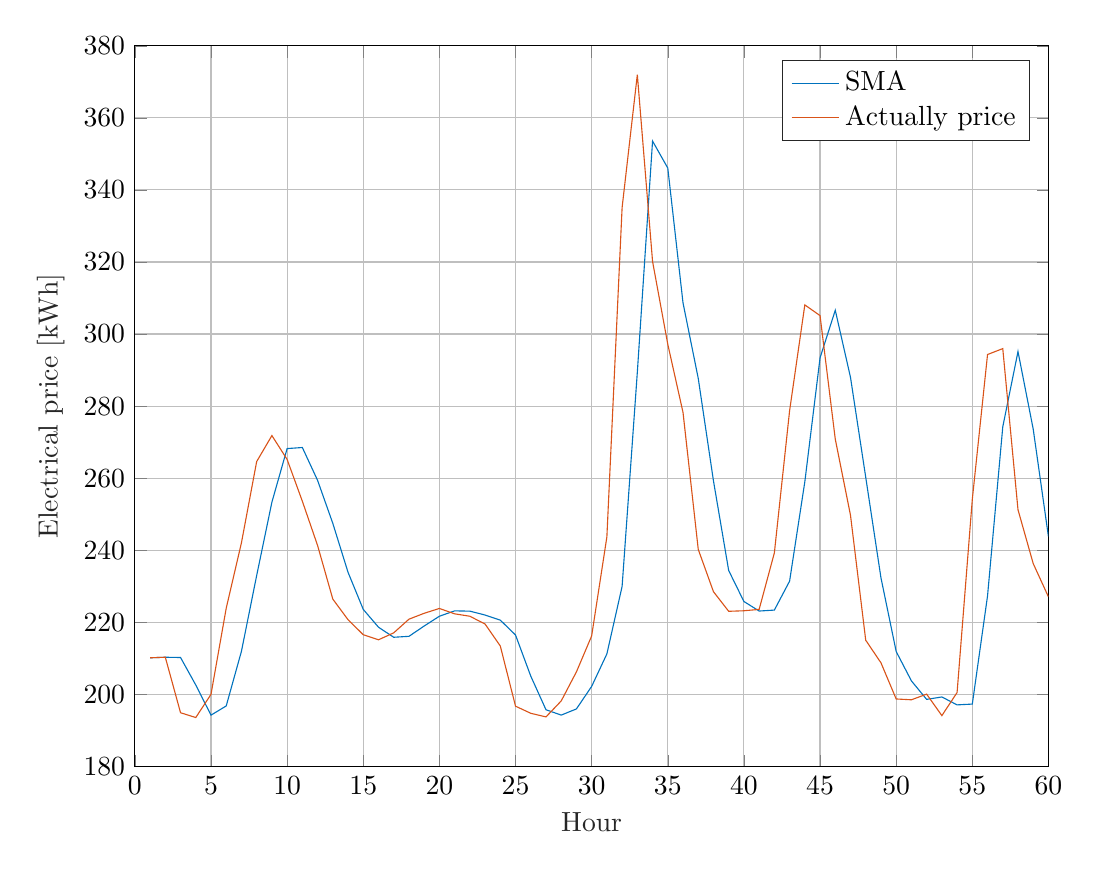
\begin{tikzpicture}

\begin{axis}[%
width=4.568in,
height=3.603in,
at={(0.766in,0.486in)},
scale only axis,
xmin=0,
xmax=60,
xlabel style={font=\color{white!15!black}},
xlabel={Hour},
ymin=180,
ymax=380,
ylabel style={font=\color{white!15!black}},
ylabel={Electrical price [kWh]},
axis background/.style={fill=white},
xmajorgrids,
ymajorgrids,
legend style={legend cell align=left, align=left, draw=white!15!black}
]
\addplot [color=mycolor1]
  table[row sep=crcr]{%
1	210.15\\
2	210.3\\
3	210.225\\
4	202.6\\
5	194.2325\\
6	196.7825\\
7	211.955\\
8	232.99\\
9	253.34\\
10	268.215\\
11	268.51\\
12	259.4\\
13	247.46\\
14	233.88\\
15	223.58\\
16	218.635\\
17	215.845\\
18	216.105\\
19	218.965\\
20	221.68\\
21	223.17\\
22	223.095\\
23	222.015\\
24	220.6\\
25	216.4725\\
26	205.0725\\
27	195.7325\\
28	194.2425\\
29	195.955\\
30	202.205\\
31	211.225\\
32	229.955\\
33	289.4\\
34	353.555\\
35	346.08\\
36	308.655\\
37	287.71\\
38	259.25\\
39	234.365\\
40	225.77\\
41	223.125\\
42	223.39\\
43	231.425\\
44	258.99\\
45	293.4\\
46	306.605\\
47	287.97\\
48	260.255\\
49	232.355\\
50	211.89\\
51	203.74\\
52	198.605\\
53	199.275\\
54	197.08\\
55	197.3\\
56	227.32\\
57	274.23\\
58	295.14\\
59	273.6\\
60	243.765\\
};
\addlegendentry{SMA}

\addplot [color=mycolor2]
  table[row sep=crcr]{%
1	210.15\\
2	210.3\\
3	194.9\\
4	193.565\\
5	200\\
6	223.91\\
7	242.07\\
8	264.61\\
9	271.82\\
10	265.2\\
11	253.6\\
12	241.32\\
13	226.44\\
14	220.72\\
15	216.55\\
16	215.14\\
17	217.07\\
18	220.86\\
19	222.5\\
20	223.84\\
21	222.35\\
22	221.68\\
23	219.52\\
24	213.425\\
25	196.72\\
26	194.745\\
27	193.74\\
28	198.17\\
29	206.24\\
30	216.21\\
31	243.7\\
32	335.1\\
33	372.01\\
34	320.15\\
35	297.16\\
36	278.26\\
37	240.24\\
38	228.49\\
39	223.05\\
40	223.2\\
41	223.58\\
42	239.27\\
43	278.71\\
44	308.09\\
45	305.12\\
46	270.82\\
47	249.69\\
48	215.02\\
49	208.76\\
50	198.72\\
51	198.49\\
52	200.06\\
53	194.1\\
54	200.5\\
55	254.14\\
56	294.32\\
57	295.96\\
58	251.24\\
59	236.29\\
60	227.06\\
};
\addlegendentry{Actually price}

\end{axis}
\end{tikzpicture}%
\caption{Two graphs that shows the price of electricity and the SMA prediction of the price.}
\label{fig:electrical_price} 
\end{figure}

It can be seen that the SMA is not a precise predictor and have a delay of two hours. However it still keeps the dynamics of the price, which is deemed enough for this project.
